\documentclass{beamer}

\mode<presentation> {
    \usetheme[compress]{Amsterdam}
    \setbeamercovered{transparent}
}

\usepackage{ucs}
\usepackage[utf8]{inputenc}
\usepackage[czech]{babel}
\usepackage{palatino}
\usepackage{graphicx}
\usepackage{epstopdf}

\usepackage{fancyvrb}
\usepackage{color}

\makeatletter
\def\PY@reset{\let\PY@it=\relax \let\PY@bf=\relax%
    \let\PY@ul=\relax \let\PY@tc=\relax%
    \let\PY@bc=\relax \let\PY@ff=\relax}
\def\PY@tok#1{\csname PY@tok@#1\endcsname}
\def\PY@toks#1+{\ifx\relax#1\empty\else%
    \PY@tok{#1}\expandafter\PY@toks\fi}
\def\PY@do#1{\PY@bc{\PY@tc{\PY@ul{%
    \PY@it{\PY@bf{\PY@ff{#1}}}}}}}
\def\PY#1#2{\PY@reset\PY@toks#1+\relax+\PY@do{#2}}

\def\PY@tok@gd{\def\PY@tc##1{\textcolor[rgb]{0.63,0.00,0.00}{##1}}}
\def\PY@tok@gu{\let\PY@bf=\textbf\def\PY@tc##1{\textcolor[rgb]{0.50,0.00,0.50}{##1}}}
\def\PY@tok@gt{\def\PY@tc##1{\textcolor[rgb]{0.00,0.25,0.82}{##1}}}
\def\PY@tok@gs{\let\PY@bf=\textbf}
\def\PY@tok@gr{\def\PY@tc##1{\textcolor[rgb]{1.00,0.00,0.00}{##1}}}
\def\PY@tok@cm{\let\PY@it=\textit\def\PY@tc##1{\textcolor[rgb]{0.25,0.50,0.50}{##1}}}
\def\PY@tok@vg{\def\PY@tc##1{\textcolor[rgb]{0.10,0.09,0.49}{##1}}}
\def\PY@tok@m{\def\PY@tc##1{\textcolor[rgb]{0.40,0.40,0.40}{##1}}}
\def\PY@tok@mh{\def\PY@tc##1{\textcolor[rgb]{0.40,0.40,0.40}{##1}}}
\def\PY@tok@go{\def\PY@tc##1{\textcolor[rgb]{0.50,0.50,0.50}{##1}}}
\def\PY@tok@ge{\let\PY@it=\textit}
\def\PY@tok@vc{\def\PY@tc##1{\textcolor[rgb]{0.10,0.09,0.49}{##1}}}
\def\PY@tok@il{\def\PY@tc##1{\textcolor[rgb]{0.40,0.40,0.40}{##1}}}
\def\PY@tok@cs{\let\PY@it=\textit\def\PY@tc##1{\textcolor[rgb]{0.25,0.50,0.50}{##1}}}
\def\PY@tok@cp{\def\PY@tc##1{\textcolor[rgb]{0.74,0.48,0.00}{##1}}}
\def\PY@tok@gi{\def\PY@tc##1{\textcolor[rgb]{0.00,0.63,0.00}{##1}}}
\def\PY@tok@gh{\let\PY@bf=\textbf\def\PY@tc##1{\textcolor[rgb]{0.00,0.00,0.50}{##1}}}
\def\PY@tok@ni{\let\PY@bf=\textbf\def\PY@tc##1{\textcolor[rgb]{0.60,0.60,0.60}{##1}}}
\def\PY@tok@nl{\def\PY@tc##1{\textcolor[rgb]{0.63,0.63,0.00}{##1}}}
\def\PY@tok@nn{\let\PY@bf=\textbf\def\PY@tc##1{\textcolor[rgb]{0.00,0.00,1.00}{##1}}}
\def\PY@tok@no{\def\PY@tc##1{\textcolor[rgb]{0.53,0.00,0.00}{##1}}}
\def\PY@tok@na{\def\PY@tc##1{\textcolor[rgb]{0.49,0.56,0.16}{##1}}}
\def\PY@tok@nb{\def\PY@tc##1{\textcolor[rgb]{0.00,0.50,0.00}{##1}}}
\def\PY@tok@nc{\let\PY@bf=\textbf\def\PY@tc##1{\textcolor[rgb]{0.00,0.00,1.00}{##1}}}
\def\PY@tok@nd{\def\PY@tc##1{\textcolor[rgb]{0.67,0.13,1.00}{##1}}}
\def\PY@tok@ne{\let\PY@bf=\textbf\def\PY@tc##1{\textcolor[rgb]{0.82,0.25,0.23}{##1}}}
\def\PY@tok@nf{\def\PY@tc##1{\textcolor[rgb]{0.00,0.00,1.00}{##1}}}
\def\PY@tok@si{\let\PY@bf=\textbf\def\PY@tc##1{\textcolor[rgb]{0.73,0.40,0.53}{##1}}}
\def\PY@tok@s2{\def\PY@tc##1{\textcolor[rgb]{0.73,0.13,0.13}{##1}}}
\def\PY@tok@vi{\def\PY@tc##1{\textcolor[rgb]{0.10,0.09,0.49}{##1}}}
\def\PY@tok@nt{\let\PY@bf=\textbf\def\PY@tc##1{\textcolor[rgb]{0.00,0.50,0.00}{##1}}}
\def\PY@tok@nv{\def\PY@tc##1{\textcolor[rgb]{0.10,0.09,0.49}{##1}}}
\def\PY@tok@s1{\def\PY@tc##1{\textcolor[rgb]{0.73,0.13,0.13}{##1}}}
\def\PY@tok@sh{\def\PY@tc##1{\textcolor[rgb]{0.73,0.13,0.13}{##1}}}
\def\PY@tok@sc{\def\PY@tc##1{\textcolor[rgb]{0.73,0.13,0.13}{##1}}}
\def\PY@tok@sx{\def\PY@tc##1{\textcolor[rgb]{0.00,0.50,0.00}{##1}}}
\def\PY@tok@bp{\def\PY@tc##1{\textcolor[rgb]{0.00,0.50,0.00}{##1}}}
\def\PY@tok@c1{\let\PY@it=\textit\def\PY@tc##1{\textcolor[rgb]{0.25,0.50,0.50}{##1}}}
\def\PY@tok@kc{\let\PY@bf=\textbf\def\PY@tc##1{\textcolor[rgb]{0.00,0.50,0.00}{##1}}}
\def\PY@tok@c{\let\PY@it=\textit\def\PY@tc##1{\textcolor[rgb]{0.25,0.50,0.50}{##1}}}
\def\PY@tok@mf{\def\PY@tc##1{\textcolor[rgb]{0.40,0.40,0.40}{##1}}}
\def\PY@tok@err{\def\PY@bc##1{\fcolorbox[rgb]{1.00,0.00,0.00}{1,1,1}{##1}}}
\def\PY@tok@kd{\let\PY@bf=\textbf\def\PY@tc##1{\textcolor[rgb]{0.00,0.50,0.00}{##1}}}
\def\PY@tok@ss{\def\PY@tc##1{\textcolor[rgb]{0.10,0.09,0.49}{##1}}}
\def\PY@tok@sr{\def\PY@tc##1{\textcolor[rgb]{0.73,0.40,0.53}{##1}}}
\def\PY@tok@mo{\def\PY@tc##1{\textcolor[rgb]{0.40,0.40,0.40}{##1}}}
\def\PY@tok@kn{\let\PY@bf=\textbf\def\PY@tc##1{\textcolor[rgb]{0.00,0.50,0.00}{##1}}}
\def\PY@tok@mi{\def\PY@tc##1{\textcolor[rgb]{0.40,0.40,0.40}{##1}}}
\def\PY@tok@gp{\let\PY@bf=\textbf\def\PY@tc##1{\textcolor[rgb]{0.00,0.00,0.50}{##1}}}
\def\PY@tok@o{\def\PY@tc##1{\textcolor[rgb]{0.40,0.40,0.40}{##1}}}
\def\PY@tok@kr{\let\PY@bf=\textbf\def\PY@tc##1{\textcolor[rgb]{0.00,0.50,0.00}{##1}}}
\def\PY@tok@s{\def\PY@tc##1{\textcolor[rgb]{0.73,0.13,0.13}{##1}}}
\def\PY@tok@kp{\def\PY@tc##1{\textcolor[rgb]{0.00,0.50,0.00}{##1}}}
\def\PY@tok@w{\def\PY@tc##1{\textcolor[rgb]{0.73,0.73,0.73}{##1}}}
\def\PY@tok@kt{\def\PY@tc##1{\textcolor[rgb]{0.69,0.00,0.25}{##1}}}
\def\PY@tok@ow{\let\PY@bf=\textbf\def\PY@tc##1{\textcolor[rgb]{0.67,0.13,1.00}{##1}}}
\def\PY@tok@sb{\def\PY@tc##1{\textcolor[rgb]{0.73,0.13,0.13}{##1}}}
\def\PY@tok@k{\let\PY@bf=\textbf\def\PY@tc##1{\textcolor[rgb]{0.00,0.50,0.00}{##1}}}
\def\PY@tok@se{\let\PY@bf=\textbf\def\PY@tc##1{\textcolor[rgb]{0.73,0.40,0.13}{##1}}}
\def\PY@tok@sd{\let\PY@it=\textit\def\PY@tc##1{\textcolor[rgb]{0.73,0.13,0.13}{##1}}}

\def\PYZbs{\char`\\}
\def\PYZus{\char`\_}
\def\PYZob{\char`\{}
\def\PYZcb{\char`\}}
\def\PYZca{\char`\^}
\def\PYZsh{\char`\#}
\def\PYZpc{\char`\%}
\def\PYZdl{\char`\$}
\def\PYZti{\char`\~}
% for compatibility with earlier versions
\def\PYZat{@}
\def\PYZlb{[}
\def\PYZrb{]}
\makeatother



\AtBeginSection[]%
{%
\begin{frame}%
  \begin{center}%
    \usebeamerfont{section title}\insertsection%
  \end{center}%
\end{frame}%
}


\title{E-puck knihovna pro Python}
\author{David Marek}
\institute[MFF UK]{Univerzita Karlova v Praze}
\date{5.~4.~2011}

\begin{document}

\begin{frame}
    \titlepage
\end{frame}

\begin{frame}
    \frametitle{Osnova}
    \tableofcontents
\end{frame}

\section{Představení e-puck robota}

\begin{frame}
    \frametitle{E-Puck}
    \begin{columns}
        \begin{column}{.6\textwidth}
            \begin{itemize}
                \item Ecole Polytechnique Fédérale de Lausanne
                \item Miniaturní robot (průměr 75mm)
                \item Opensource hardware
                \item Spousta senzorů
                \item Bluetooth komunikace
                \item Dostupný (v labu)
            \end{itemize}
        \end{column}

        \begin{column}{.4\textwidth}
            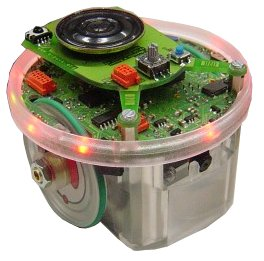
\includegraphics[scale=0.4]{e-puck.jpg}
        \end{column}
    \end{columns}
\end{frame}


\begin{frame}
    \frametitle{Senzory a akční členy}
    \begin{itemize}
        \item Kamera (640x480)
        \item IR senzory (proximity / ambient light)
        \item Akcelerometr (3D)
        \item Mikrofony
        \item LED
        \item Krokové motory
        \item Speaker
    \end{itemize}
\end{frame}

\begin{frame}
    \frametitle{Kamera}
    \begin{columns}
        \begin{column}{.7\textwidth}
            \begin{itemize}
                \item Rozlišení 640x480
                \item Dva režimy: RGB565 / barvy šedi
                \item Příliš velké fotky pro zpracování v robotovi
                \item Řešení problémů s pamětí:
                    \begin{itemize}
                        \item Prokládání
                        \item Změna formátu fotografie
                    \end{itemize}
                \item Reálně jde získat:
                    \begin{itemize}
                        \item 40x40 barevně
                        \item 55x55 černobíle
                        \item Lineární kamera
                    \end{itemize}
            \end{itemize}
        \end{column}

        \begin{column}[c]{.3\textwidth}
            \begin{center}
                \hspace{-2cm}
\includegraphics{fotka1.jpg}\\
                \vspace{0.3cm}
                \hspace{-2cm}
\includegraphics{fotka2.jpg}\\
                \vspace{0.3cm}
                \hspace{-2cm}
\includegraphics{fotka3.jpg}\\
                \vspace{0.3cm}
                \hspace{-2cm}
\includegraphics[scale=0.4]{fotka4.jpg}
            \end{center}
        \end{column}
    \end{columns}
\end{frame}

\begin{frame}
    \frametitle{IR senzory}
    \begin{columns}
        \begin{column}{0.6\textwidth}
            \begin{itemize}
                \item 8 senzorů po obvodu
                \item Dva režimy:
                    \begin{itemize}
                        \item Aktivní -- rozeznávání překážek
                        \item Pasivní -- intenzita světla
                    \end{itemize}
                \item Překážky do $\sim$ 4cm
            \end{itemize}
        \end{column}

        \begin{column}{0.4\textwidth}
            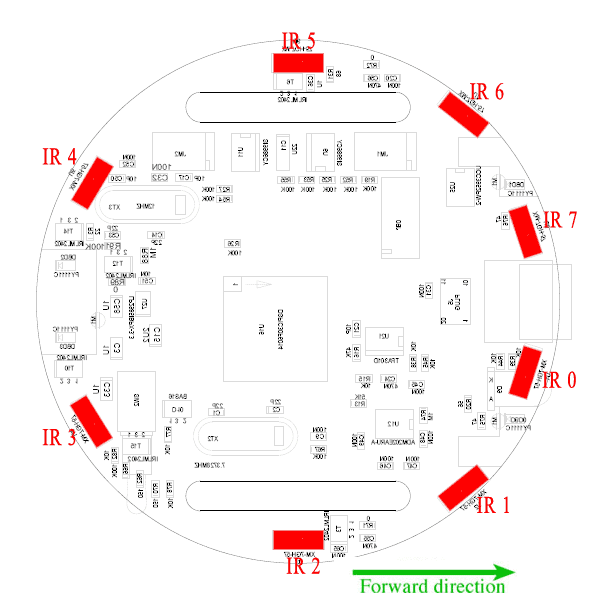
\includegraphics[scale=0.2]{proximity_emplacement.png}
        \end{column}
    \end{columns}
\end{frame}

\begin{frame}
    \frametitle{Akcelerometr}
    \begin{columns}
        \begin{column}{0.6\textwidth}
            \begin{itemize}
                \item 3D akcelerometr
                \item Z robota se dá získat:
                    \begin{itemize}
                        \item Vektor akcelerace
                        \item Zpracované informace (rotace, zrychlení, \ldots)
                    \end{itemize}
                \item Detekce nárazu, naklonění, směru pohybu
            \end{itemize}
        \end{column}

        \begin{column}{0.4\textwidth}
            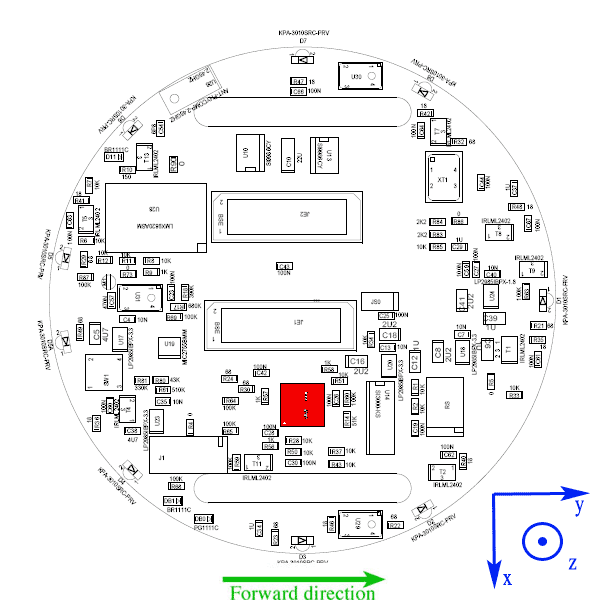
\includegraphics[scale=0.2]{acc_emplacement.png}
        \end{column}
    \end{columns}
\end{frame}

\begin{frame}
    \frametitle{Mikrofony}
    \begin{columns}
        \begin{column}{0.6\textwidth}
            \begin{itemize}
                \item 3 mikrofony
                \item Vlevo, vpravo, vzadu
                \item Lze získat:
                \begin{itemize}
                    \item Hlasitost
                    \item Frekvenci (FFT)
                \end{itemize}
            \end{itemize}
        \end{column}

        \begin{column}{0.4\textwidth}
            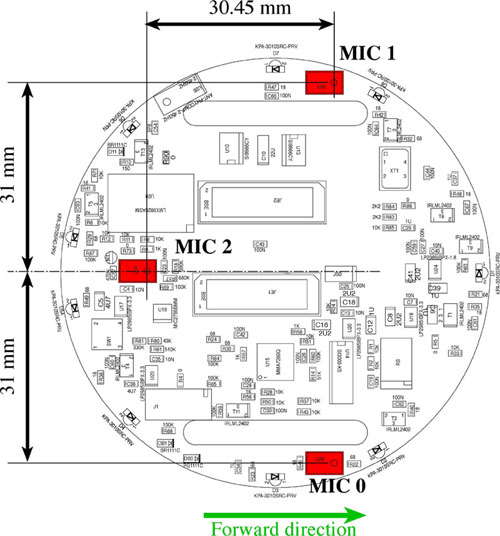
\includegraphics[scale=1]{sound.jpg}
        \end{column}
    \end{columns}
\end{frame}

\begin{frame}
    \frametitle{LED}
    \begin{columns}
        \begin{column}{0.5\textwidth}
            \begin{itemize}
                \item 8 LED po obvodu robota
                \item Zelená dioda v těle robota
                \item Jasná dioda u kamery
            \end{itemize}
        \end{column}

        \begin{column}{0.5\textwidth}
            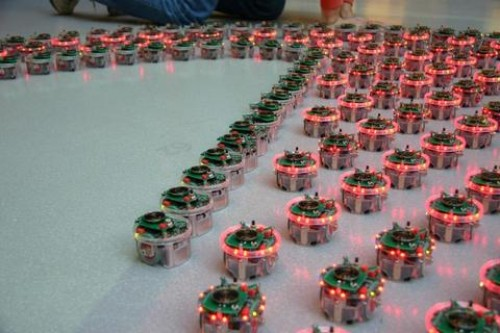
\includegraphics[scale=0.3]{e-puck_3.JPG}
        \end{column}
    \end{columns}
\end{frame}

\begin{frame}
    \frametitle{Krokové motory}
    \begin{columns}
        \begin{column}{0.5\textwidth}
            \begin{itemize}
                \item Dva krokové motory
                \item Tisíc kroků = jedna otáčka kola
                \item Jeden krok $\approx$ 0.13 mm
                \item Maximální rychlost jedna otáčka za sekundu
                \item Neklouzavá úprava
            \end{itemize}
        \end{column}

        \begin{column}{0.5\textwidth}
            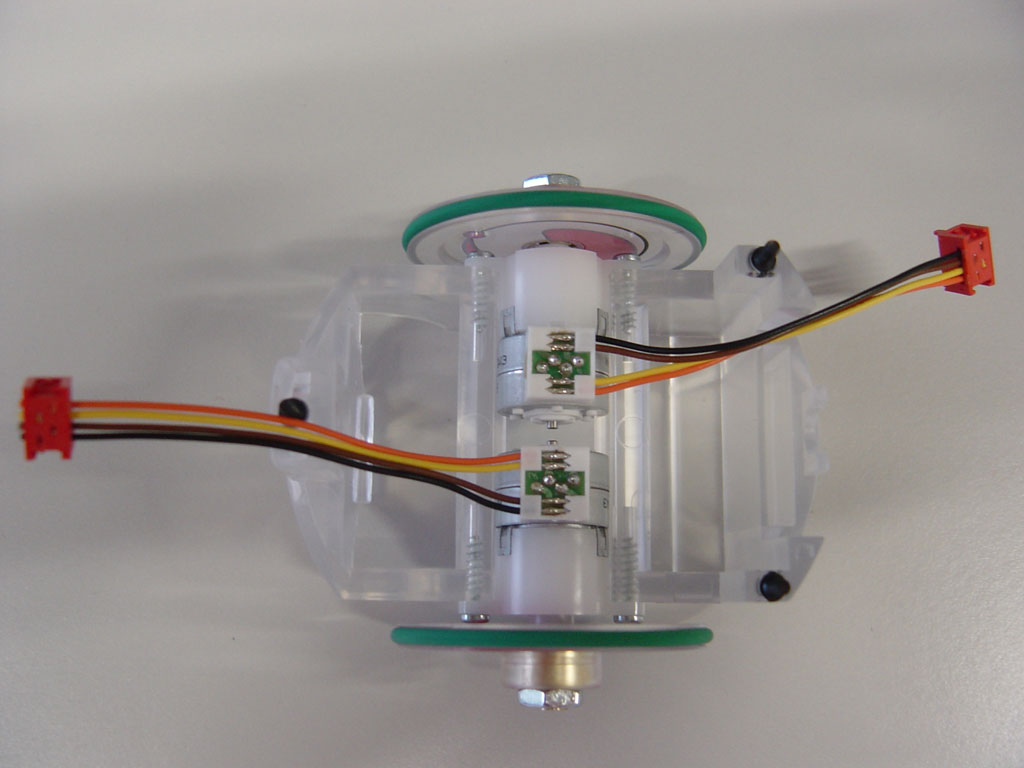
\includegraphics[scale=0.15]{mecanics.jpg}
        \end{column}
    \end{columns}
\end{frame}

\begin{frame}
    \frametitle{Speaker}
        \begin{itemize}
            \item Přehrává připravené zvuky (WAV)
            \item 5 zvuků zakompilovaných do firmware
        \end{itemize}
\end{frame}

\section{Připojení}

\begin{frame}
    \frametitle{Příprava PC}
    \begin{itemize}
        \item Potřeba funkční bluetooth
        \item Balíky {\tt bluez-firmware}, {\tt bluez-utils}
        \item Utilita na zaslání PIN ({\tt bluez-pin}, \ldots)
    \end{itemize}
\end{frame}

\begin{frame}[fragile]
    \frametitle{Nastavení rfcomm}
    \begin{block}{Získat adresu robota}
    \begin{Verbatim}[commandchars=\\\{\}]
\PY{n+nv}{\PYZdl{} }hcitool scan
Scanning ...
	10:00:E8:52:C6:3E	e-puck\PYZus{}1055
\end{Verbatim}
    \end{block}

    \begin{block}{Nastavení {\tt /etc/bluetooth/rfcomm.conf}}
\begin{Verbatim}[commandchars=\\\{\}]
\PY{l+lScalar+lScalarPlain}{rfcomm2}\PY{l+lScalar+lScalarPlain}{ }\PY{l+lScalar+lScalarPlain}{\PYZob{}}
    \PY{l+lScalar+lScalarPlain}{bind}\PY{l+lScalar+lScalarPlain}{ }\PY{l+lScalar+lScalarPlain}{yes;}
    \PY{l+lScalar+lScalarPlain}{device}\PY{l+lScalar+lScalarPlain}{ }\PY{l+lScalar+lScalarPlain}{10:00:E8:52:C6:3E;} \PY{c+c1}{\PYZsh{} Adresa z hcitool}
    \PY{l+lScalar+lScalarPlain}{channel}\PY{l+lScalar+lScalarPlain}{ }\PY{l+lScalar+lScalarPlain}{1;}
    \PY{l+lScalar+lScalarPlain}{comment}\PY{l+lScalar+lScalarPlain}{ }\PY{l+lScalar+lScalarPlain}{"e-puck\PYZus{}1055";}    \PY{c+c1}{\PYZsh{} Komentář}
{\PYZcb{}}
\end{Verbatim}

    \end{block}
\end{frame}

\begin{frame}[fragile]
    \frametitle{Vytvoření spojení}
    \begin{block}{Připojení pomocí {\tt rfcomm}}
    \begin{Verbatim}[fontsize=\small]
# rfcomm connect rfcomm2
Connected /dev/rfcomm2 to 10:00:E8:52:C6:3E on channel 1
Press CTRL-C for hangup
    \end{Verbatim}
    \end{block}

    \begin{alertblock}{Možné chyby}
        {\em Can’t connect RFCOMM socket: Connection refused}
        \begin{itemize}
            \item Není spuštěná aplikace, která by předala PIN
        \end{itemize}
        {\em Can’t create RFCOMM TTY: Address already in use}
        \begin{itemize}
            \item Robot už je připojen
            \item Jiná aplikace s ním stále komunikuje
        \end{itemize}
    \end{alertblock}
\end{frame}

\begin{frame}[fragile]
    \frametitle{Nahrání firmware}
    \begin{itemize}
        \item Používá se {\tt epuckupload}
        \item Je potřeba mít aktivní připojení
        \item Robot dokáže přijímat nový firmware pouze pár sekund po restartu
    \end{itemize}
    \begin{block}{Postup při nahrávání}
        \begin{enumerate}
            \item Spuštění nahrávání
\begin{Verbatim}[commandchars=\\\{\}]
\PY{n+nv}{\PYZdl{} }epuckupload -f BTcom.hex rfcomm2
\end{Verbatim}
            \item Restartování robota
            \item Vyčkání na konec nahrávání
            \item Robot připraven k práci
        \end{enumerate}
    \end{block}

\end{frame}

\section{Komunikace}

\begin{frame}
    \begin{itemize}
        \item Pokus
    \end{itemize}
\end{frame}


\begin{frame}
    \begin{itemize}
        \item Pokus
    \end{itemize}
\end{frame}


\begin{frame}
    \begin{itemize}
        \item Pokus
    \end{itemize}
\end{frame}

\section{Přehled příkazů}

\begin{frame}
    \begin{itemize}
        \item Pokus
    \end{itemize}
\end{frame}

\section{Ukázky programů}

\begin{frame}
    \begin{itemize}
        \item Pokus
    \end{itemize}
\end{frame}


\end{document}
